\documentclass[twoside]{book}

% Packages required by doxygen
\usepackage{fixltx2e}
\usepackage{calc}
\usepackage{doxygen}
\usepackage[export]{adjustbox} % also loads graphicx
\usepackage{graphicx}
\usepackage[utf8]{inputenc}
\usepackage{makeidx}
\usepackage{multicol}
\usepackage{multirow}
\PassOptionsToPackage{warn}{textcomp}
\usepackage{textcomp}
\usepackage[nointegrals]{wasysym}
\usepackage[table]{xcolor}

% Font selection
\usepackage[T1]{fontenc}
\usepackage[scaled=.90]{helvet}
\usepackage{courier}
\usepackage{amssymb}
\usepackage{sectsty}
\renewcommand{\familydefault}{\sfdefault}
\allsectionsfont{%
  \fontseries{bc}\selectfont%
  \color{darkgray}%
}
\renewcommand{\DoxyLabelFont}{%
  \fontseries{bc}\selectfont%
  \color{darkgray}%
}
\newcommand{\+}{\discretionary{\mbox{\scriptsize$\hookleftarrow$}}{}{}}

% Page & text layout
\usepackage{geometry}
\geometry{%
  a4paper,%
  top=2.5cm,%
  bottom=2.5cm,%
  left=2.5cm,%
  right=2.5cm%
}
\tolerance=750
\hfuzz=15pt
\hbadness=750
\setlength{\emergencystretch}{15pt}
\setlength{\parindent}{0cm}
\setlength{\parskip}{3ex plus 2ex minus 2ex}
\makeatletter
\renewcommand{\paragraph}{%
  \@startsection{paragraph}{4}{0ex}{-1.0ex}{1.0ex}{%
    \normalfont\normalsize\bfseries\SS@parafont%
  }%
}
\renewcommand{\subparagraph}{%
  \@startsection{subparagraph}{5}{0ex}{-1.0ex}{1.0ex}{%
    \normalfont\normalsize\bfseries\SS@subparafont%
  }%
}
\makeatother

% Headers & footers
\usepackage{fancyhdr}
\pagestyle{fancyplain}
\fancyhead[LE]{\fancyplain{}{\bfseries\thepage}}
\fancyhead[CE]{\fancyplain{}{}}
\fancyhead[RE]{\fancyplain{}{\bfseries\leftmark}}
\fancyhead[LO]{\fancyplain{}{\bfseries\rightmark}}
\fancyhead[CO]{\fancyplain{}{}}
\fancyhead[RO]{\fancyplain{}{\bfseries\thepage}}
\fancyfoot[LE]{\fancyplain{}{}}
\fancyfoot[CE]{\fancyplain{}{}}
\fancyfoot[RE]{\fancyplain{}{\bfseries\scriptsize Generated by Doxygen }}
\fancyfoot[LO]{\fancyplain{}{\bfseries\scriptsize Generated by Doxygen }}
\fancyfoot[CO]{\fancyplain{}{}}
\fancyfoot[RO]{\fancyplain{}{}}
\renewcommand{\footrulewidth}{0.4pt}
\renewcommand{\chaptermark}[1]{%
  \markboth{#1}{}%
}
\renewcommand{\sectionmark}[1]{%
  \markright{\thesection\ #1}%
}

% Indices & bibliography
\usepackage{natbib}
\usepackage[titles]{tocloft}
\setcounter{tocdepth}{3}
\setcounter{secnumdepth}{5}
\makeindex

% Hyperlinks (required, but should be loaded last)
\usepackage{ifpdf}
\ifpdf
  \usepackage[pdftex,pagebackref=true]{hyperref}
\else
  \usepackage[ps2pdf,pagebackref=true]{hyperref}
\fi
\hypersetup{%
  colorlinks=true,%
  linkcolor=blue,%
  citecolor=blue,%
  unicode%
}

% Custom commands
\newcommand{\clearemptydoublepage}{%
  \newpage{\pagestyle{empty}\cleardoublepage}%
}

\usepackage{caption}
\captionsetup{labelsep=space,justification=centering,font={bf},singlelinecheck=off,skip=4pt,position=top}

%===== C O N T E N T S =====

\begin{document}

% Titlepage & ToC
\hypersetup{pageanchor=false,
             bookmarksnumbered=true,
             pdfencoding=unicode
            }
\pagenumbering{alph}
\begin{titlepage}
\vspace*{7cm}
\begin{center}%
{\Large My Project }\\
\vspace*{1cm}
{\large Generated by Doxygen 1.8.13}\\
\end{center}
\end{titlepage}
\clearemptydoublepage
\pagenumbering{roman}
\tableofcontents
\clearemptydoublepage
\pagenumbering{arabic}
\hypersetup{pageanchor=true}

%--- Begin generated contents ---
\chapter{Drone Search and Rescue}
\label{index}\hypertarget{index}{}\hypertarget{index_intro_sec}{}\section{Introduction}\label{index_intro_sec}
Canny edge detection is a multi-\/step image filter that detects only the outlines of an image. It is the culmination of 6 individual filters, applied one after another until only the edges of the original image are pronounced.\hypertarget{index_how_works_sec}{}\section{How it Works\+:}\label{index_how_works_sec}
Each of the below filters are applied to an image. Starting with a Greyscale \hyperlink{classFilter}{Filter} and ending with a Hysteresis \hyperlink{classFilter}{Filter}. The resulting image is a Canny Edge Detection Filtered image.


\begin{DoxyEnumerate}
\item Greyscale
\item Gaussian blur
\item Sobel filter
\item Non-\/max suppression
\item Double threshold
\item Hysteresis
\end{DoxyEnumerate}
\chapter{Hierarchical Index}
\section{Class Hierarchy}
This inheritance list is sorted roughly, but not completely, alphabetically\+:\begin{DoxyCompactList}
\item \contentsline{section}{Filter}{\pageref{classFilter}}{}
\begin{DoxyCompactList}
\item \contentsline{section}{Double\+Threshold\+Filter}{\pageref{classDoubleThresholdFilter}}{}
\item \contentsline{section}{Grey\+Scale\+Filter}{\pageref{classGreyScaleFilter}}{}
\item \contentsline{section}{Hysteresis\+Filter}{\pageref{classHysteresisFilter}}{}
\end{DoxyCompactList}
\item \contentsline{section}{Image}{\pageref{classImage}}{}
\item \contentsline{section}{stbi\+\_\+io\+\_\+callbacks}{\pageref{structstbi__io__callbacks}}{}
\end{DoxyCompactList}

\chapter{Class Index}
\section{Class List}
Here are the classes, structs, unions and interfaces with brief descriptions\+:\begin{DoxyCompactList}
\item\contentsline{section}{\hyperlink{classBeeline}{Beeline} \\*The class for moving the drone in a straight line from point A to point B }{\pageref{classBeeline}}{}
\item\contentsline{section}{\hyperlink{classDrone}{Drone} \\*The class for representing the drone object in the simulation }{\pageref{classDrone}}{}
\item\contentsline{section}{\hyperlink{classEntityFactory}{Entity\+Factory} \\*The class for creating json object entities }{\pageref{classEntityFactory}}{}
\item\contentsline{section}{\hyperlink{classMovement}{Movement} \\*The class for handling movement of the drone }{\pageref{classMovement}}{}
\item\contentsline{section}{\hyperlink{classSimulation}{Simulation} \\*The class for simulating a drone finding a robot }{\pageref{classSimulation}}{}
\item\contentsline{section}{\hyperlink{classWebApp}{Web\+App} \\*A Web Application Sever that communicates with a web page through web sockets }{\pageref{classWebApp}}{}
\end{DoxyCompactList}

\chapter{Class Documentation}
\hypertarget{classBeeline}{}\section{Beeline Class Reference}
\label{classBeeline}\index{Beeline@{Beeline}}


The class for moving the drone in a straight line from point A to point B.  




{\ttfamily \#include $<$beeline.\+h$>$}



Inheritance diagram for Beeline\+:\nopagebreak
\begin{figure}[H]
\begin{center}
\leavevmode
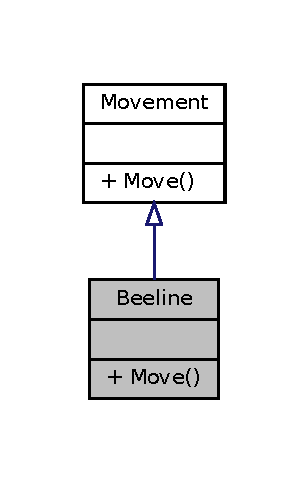
\includegraphics[width=148pt]{classBeeline__inherit__graph}
\end{center}
\end{figure}


Collaboration diagram for Beeline\+:\nopagebreak
\begin{figure}[H]
\begin{center}
\leavevmode
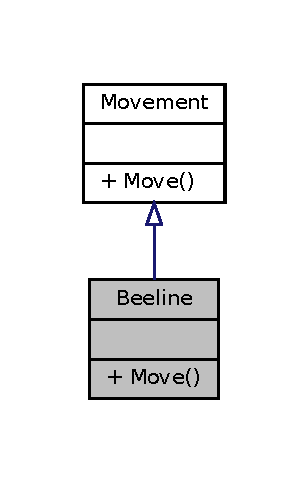
\includegraphics[width=148pt]{classBeeline__coll__graph}
\end{center}
\end{figure}
\subsection*{Public Member Functions}
\begin{DoxyCompactItemize}
\item 
\mbox{\Hypertarget{classBeeline_af53d1b01ae714fa2cd61f5a053165ca1}\label{classBeeline_af53d1b01ae714fa2cd61f5a053165ca1}} 
void \hyperlink{classBeeline_af53d1b01ae714fa2cd61f5a053165ca1}{Move} (\hyperlink{classDrone}{Drone} \&drone, double direction\mbox{[}3\mbox{]}, double distance, float speed, double dt)
\begin{DoxyCompactList}\small\item\em Moves the drone in straight line. \end{DoxyCompactList}\end{DoxyCompactItemize}


\subsection{Detailed Description}
The class for moving the drone in a straight line from point A to point B. 

The documentation for this class was generated from the following files\+:\begin{DoxyCompactItemize}
\item 
/home/user/repo/project/src/beeline.\+h\item 
/home/user/repo/project/src/beeline.\+cc\end{DoxyCompactItemize}

\hypertarget{classDrone}{}\section{Drone Class Reference}
\label{classDrone}\index{Drone@{Drone}}


The class for representing the drone object in the simulation.  




{\ttfamily \#include $<$drone.\+h$>$}



Inheritance diagram for Drone\+:\nopagebreak
\begin{figure}[H]
\begin{center}
\leavevmode
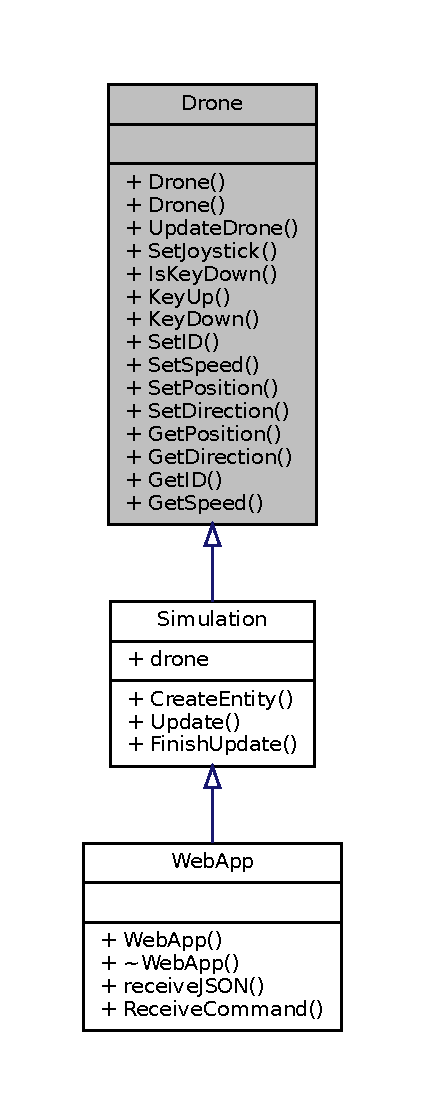
\includegraphics[width=204pt]{classDrone__inherit__graph}
\end{center}
\end{figure}


Collaboration diagram for Drone\+:\nopagebreak
\begin{figure}[H]
\begin{center}
\leavevmode
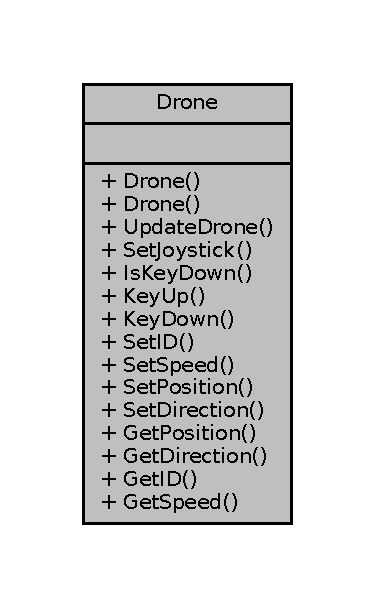
\includegraphics[width=180pt]{classDrone__coll__graph}
\end{center}
\end{figure}
\subsection*{Public Member Functions}
\begin{DoxyCompactItemize}
\item 
\mbox{\Hypertarget{classDrone_ab692baa4be5c43b72990ce1b01bdc805}\label{classDrone_ab692baa4be5c43b72990ce1b01bdc805}} 
\hyperlink{classDrone_ab692baa4be5c43b72990ce1b01bdc805}{Drone} ()
\begin{DoxyCompactList}\small\item\em Default drone constructor. \end{DoxyCompactList}\item 
\mbox{\Hypertarget{classDrone_a7875422c0bf36072ab6d747b6d543b67}\label{classDrone_a7875422c0bf36072ab6d747b6d543b67}} 
\hyperlink{classDrone_a7875422c0bf36072ab6d747b6d543b67}{Drone} (double x, double y, double z)
\begin{DoxyCompactList}\small\item\em Construct a drone at a given position. \end{DoxyCompactList}\item 
\mbox{\Hypertarget{classDrone_ad8b728197d7de13358f17e192a9c7e1d}\label{classDrone_ad8b728197d7de13358f17e192a9c7e1d}} 
void \hyperlink{classDrone_ad8b728197d7de13358f17e192a9c7e1d}{Update\+Drone} (double dt)
\begin{DoxyCompactList}\small\item\em Updates the drone position and other dynamic properties. \end{DoxyCompactList}\item 
\mbox{\Hypertarget{classDrone_a49ba636e2a579845fbc85eda05ea3735}\label{classDrone_a49ba636e2a579845fbc85eda05ea3735}} 
void \hyperlink{classDrone_a49ba636e2a579845fbc85eda05ea3735}{Set\+Joystick} (double x, double y, double z, double a)
\begin{DoxyCompactList}\small\item\em Sets the direction of the drone. \end{DoxyCompactList}\item 
bool \hyperlink{classDrone_a9b164e1535a80ce8e4de11ab0c0edcdc}{Is\+Key\+Down} (const std\+::string \&key)
\begin{DoxyCompactList}\small\item\em Check if keys are pressed. \end{DoxyCompactList}\item 
\mbox{\Hypertarget{classDrone_a95aca396f093db8ec2a8e533e6a8bd60}\label{classDrone_a95aca396f093db8ec2a8e533e6a8bd60}} 
void \hyperlink{classDrone_a95aca396f093db8ec2a8e533e6a8bd60}{Key\+Up} (const std\+::string \&key, int key\+Code)
\begin{DoxyCompactList}\small\item\em Sets the key\+Value indexed at key to 0. \end{DoxyCompactList}\item 
\mbox{\Hypertarget{classDrone_a83a6384bcefa360055df86dca5ec3afc}\label{classDrone_a83a6384bcefa360055df86dca5ec3afc}} 
void \hyperlink{classDrone_a83a6384bcefa360055df86dca5ec3afc}{Key\+Down} (const std\+::string \&key, int key\+Code)
\begin{DoxyCompactList}\small\item\em Sets the key\+Value indexed at key to 1. \end{DoxyCompactList}\item 
\mbox{\Hypertarget{classDrone_ad2ad45f67c4c74a2364d09b5cccb991d}\label{classDrone_ad2ad45f67c4c74a2364d09b5cccb991d}} 
void \hyperlink{classDrone_ad2ad45f67c4c74a2364d09b5cccb991d}{Set\+ID} (int i)
\begin{DoxyCompactList}\small\item\em Sets the drone\textquotesingle{}s ID. \end{DoxyCompactList}\item 
\mbox{\Hypertarget{classDrone_a84fd5637a4a226c39c3ad3cd256c77e2}\label{classDrone_a84fd5637a4a226c39c3ad3cd256c77e2}} 
void \hyperlink{classDrone_a84fd5637a4a226c39c3ad3cd256c77e2}{Set\+Speed} (double s)
\begin{DoxyCompactList}\small\item\em Sets the drone\textquotesingle{}s speed. \end{DoxyCompactList}\item 
\mbox{\Hypertarget{classDrone_aceb8b8df70fd3e70a6fc1cc8fefe9512}\label{classDrone_aceb8b8df70fd3e70a6fc1cc8fefe9512}} 
void \hyperlink{classDrone_aceb8b8df70fd3e70a6fc1cc8fefe9512}{Set\+Position} (double x, double y, double z)
\begin{DoxyCompactList}\small\item\em Sets the drone\textquotesingle{}s position. \end{DoxyCompactList}\item 
\mbox{\Hypertarget{classDrone_a45a3478122b291066f9cbd80533a686b}\label{classDrone_a45a3478122b291066f9cbd80533a686b}} 
void \hyperlink{classDrone_a45a3478122b291066f9cbd80533a686b}{Set\+Direction} (double x, double y, double z)
\begin{DoxyCompactList}\small\item\em Sets the drone\textquotesingle{}s direction. \end{DoxyCompactList}\item 
double \hyperlink{classDrone_ad8e2a72eb608ef4f8a82402a74fd5ad5}{Get\+Position} (int index)
\begin{DoxyCompactList}\small\item\em Gets the drone\textquotesingle{}s position at a given index. \end{DoxyCompactList}\item 
double \hyperlink{classDrone_a3c240b2f2cb2a355f27e31dd3b5ac931}{Get\+Direction} (int index)
\begin{DoxyCompactList}\small\item\em Gets the drone\textquotesingle{}s direction at a given index. \end{DoxyCompactList}\item 
int \hyperlink{classDrone_a5e69f5ebe80ece53ccb2238a2b598d97}{Get\+ID} ()
\begin{DoxyCompactList}\small\item\em Gets the drone\textquotesingle{}s ID. \end{DoxyCompactList}\item 
double \hyperlink{classDrone_ac8c535643f2be526c0ac8b0cc1fc49fc}{Get\+Speed} ()
\begin{DoxyCompactList}\small\item\em Gets the drone\textquotesingle{}s speed. \end{DoxyCompactList}\end{DoxyCompactItemize}


\subsection{Detailed Description}
The class for representing the drone object in the simulation. 

\subsection{Member Function Documentation}
\mbox{\Hypertarget{classDrone_a3c240b2f2cb2a355f27e31dd3b5ac931}\label{classDrone_a3c240b2f2cb2a355f27e31dd3b5ac931}} 
\index{Drone@{Drone}!Get\+Direction@{Get\+Direction}}
\index{Get\+Direction@{Get\+Direction}!Drone@{Drone}}
\subsubsection{\texorpdfstring{Get\+Direction()}{GetDirection()}}
{\footnotesize\ttfamily double Drone\+::\+Get\+Direction (\begin{DoxyParamCaption}\item[{int}]{index }\end{DoxyParamCaption})\hspace{0.3cm}{\ttfamily [inline]}}



Gets the drone\textquotesingle{}s direction at a given index. 

\begin{DoxyReturn}{Returns}
The drone\textquotesingle{}s direction at a given index 
\end{DoxyReturn}
\mbox{\Hypertarget{classDrone_a5e69f5ebe80ece53ccb2238a2b598d97}\label{classDrone_a5e69f5ebe80ece53ccb2238a2b598d97}} 
\index{Drone@{Drone}!Get\+ID@{Get\+ID}}
\index{Get\+ID@{Get\+ID}!Drone@{Drone}}
\subsubsection{\texorpdfstring{Get\+I\+D()}{GetID()}}
{\footnotesize\ttfamily int Drone\+::\+Get\+ID (\begin{DoxyParamCaption}{ }\end{DoxyParamCaption})\hspace{0.3cm}{\ttfamily [inline]}}



Gets the drone\textquotesingle{}s ID. 

\begin{DoxyReturn}{Returns}
The drone\textquotesingle{}s ID 
\end{DoxyReturn}
\mbox{\Hypertarget{classDrone_ad8e2a72eb608ef4f8a82402a74fd5ad5}\label{classDrone_ad8e2a72eb608ef4f8a82402a74fd5ad5}} 
\index{Drone@{Drone}!Get\+Position@{Get\+Position}}
\index{Get\+Position@{Get\+Position}!Drone@{Drone}}
\subsubsection{\texorpdfstring{Get\+Position()}{GetPosition()}}
{\footnotesize\ttfamily double Drone\+::\+Get\+Position (\begin{DoxyParamCaption}\item[{int}]{index }\end{DoxyParamCaption})\hspace{0.3cm}{\ttfamily [inline]}}



Gets the drone\textquotesingle{}s position at a given index. 

\begin{DoxyReturn}{Returns}
The drone\textquotesingle{}s position at a given index 
\end{DoxyReturn}
\mbox{\Hypertarget{classDrone_ac8c535643f2be526c0ac8b0cc1fc49fc}\label{classDrone_ac8c535643f2be526c0ac8b0cc1fc49fc}} 
\index{Drone@{Drone}!Get\+Speed@{Get\+Speed}}
\index{Get\+Speed@{Get\+Speed}!Drone@{Drone}}
\subsubsection{\texorpdfstring{Get\+Speed()}{GetSpeed()}}
{\footnotesize\ttfamily double Drone\+::\+Get\+Speed (\begin{DoxyParamCaption}{ }\end{DoxyParamCaption})\hspace{0.3cm}{\ttfamily [inline]}}



Gets the drone\textquotesingle{}s speed. 

\begin{DoxyReturn}{Returns}
The drone\textquotesingle{}s speed 
\end{DoxyReturn}
\mbox{\Hypertarget{classDrone_a9b164e1535a80ce8e4de11ab0c0edcdc}\label{classDrone_a9b164e1535a80ce8e4de11ab0c0edcdc}} 
\index{Drone@{Drone}!Is\+Key\+Down@{Is\+Key\+Down}}
\index{Is\+Key\+Down@{Is\+Key\+Down}!Drone@{Drone}}
\subsubsection{\texorpdfstring{Is\+Key\+Down()}{IsKeyDown()}}
{\footnotesize\ttfamily bool Drone\+::\+Is\+Key\+Down (\begin{DoxyParamCaption}\item[{const std\+::string \&}]{key }\end{DoxyParamCaption})}



Check if keys are pressed. 

\begin{DoxyReturn}{Returns}
True if yes, False if not 
\end{DoxyReturn}


The documentation for this class was generated from the following files\+:\begin{DoxyCompactItemize}
\item 
/home/user/repo/project/src/drone.\+h\item 
/home/user/repo/project/src/drone.\+cc\end{DoxyCompactItemize}

\hypertarget{classEntityFactory}{}\section{Entity\+Factory Class Reference}
\label{classEntityFactory}\index{Entity\+Factory@{Entity\+Factory}}


The class for creating json object entities.  




{\ttfamily \#include $<$entity\+\_\+factory.\+h$>$}



Inheritance diagram for Entity\+Factory\+:\nopagebreak
\begin{figure}[H]
\begin{center}
\leavevmode
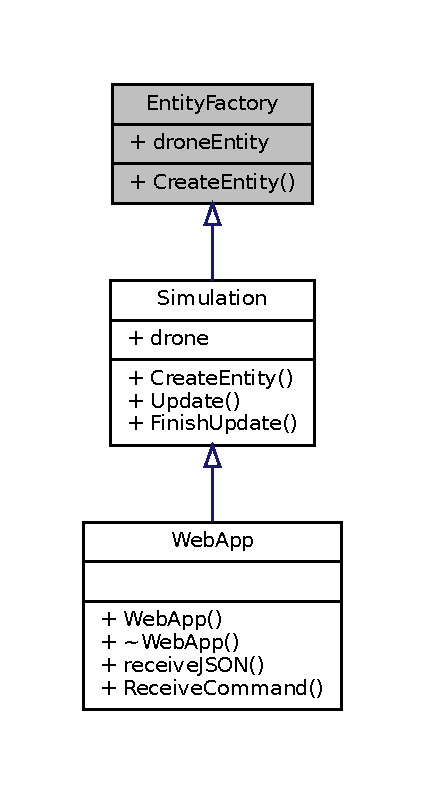
\includegraphics[width=204pt]{classEntityFactory__inherit__graph}
\end{center}
\end{figure}


Collaboration diagram for Entity\+Factory\+:\nopagebreak
\begin{figure}[H]
\begin{center}
\leavevmode
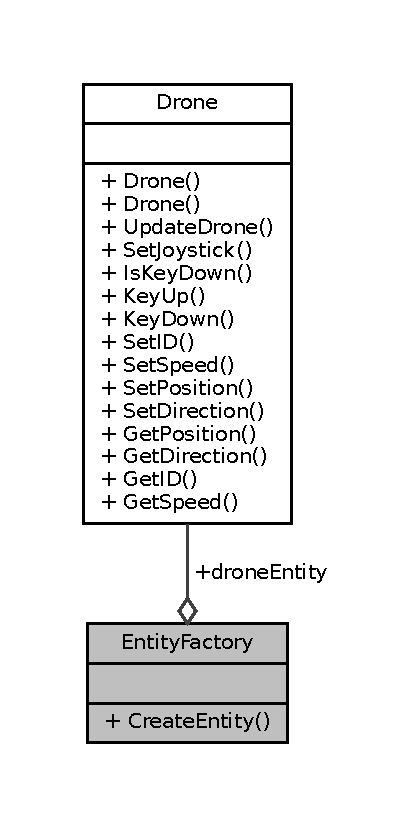
\includegraphics[width=198pt]{classEntityFactory__coll__graph}
\end{center}
\end{figure}
\subsection*{Public Member Functions}
\begin{DoxyCompactItemize}
\item 
\mbox{\Hypertarget{classEntityFactory_a4be383d4c4efb17ae4cff9c27b84c47c}\label{classEntityFactory_a4be383d4c4efb17ae4cff9c27b84c47c}} 
void \hyperlink{classEntityFactory_a4be383d4c4efb17ae4cff9c27b84c47c}{Create\+Entity} (picojson\+::object \&entity\+Data)
\begin{DoxyCompactList}\small\item\em Creates an entity based on the object passed in. \end{DoxyCompactList}\end{DoxyCompactItemize}
\subsection*{Public Attributes}
\begin{DoxyCompactItemize}
\item 
\mbox{\Hypertarget{classEntityFactory_a467ebf6906f2410bf3574f29c4c0de61}\label{classEntityFactory_a467ebf6906f2410bf3574f29c4c0de61}} 
\hyperlink{classDrone}{Drone} {\bfseries drone\+Entity}
\end{DoxyCompactItemize}


\subsection{Detailed Description}
The class for creating json object entities. 

The documentation for this class was generated from the following files\+:\begin{DoxyCompactItemize}
\item 
/home/user/repo/project/src/entity\+\_\+factory.\+h\item 
/home/user/repo/project/src/entity\+\_\+factory.\+cc\end{DoxyCompactItemize}

\hypertarget{classMovement}{}\section{Movement Class Reference}
\label{classMovement}\index{Movement@{Movement}}


The class for handling movement of the drone.  




{\ttfamily \#include $<$movement.\+h$>$}



Inheritance diagram for Movement\+:\nopagebreak
\begin{figure}[H]
\begin{center}
\leavevmode
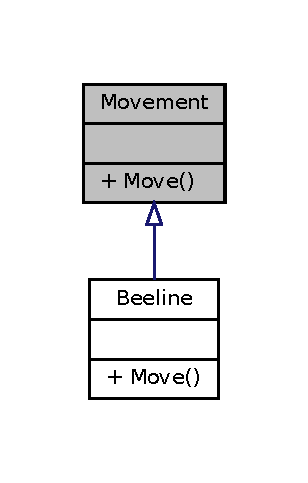
\includegraphics[width=148pt]{classMovement__inherit__graph}
\end{center}
\end{figure}


Collaboration diagram for Movement\+:\nopagebreak
\begin{figure}[H]
\begin{center}
\leavevmode
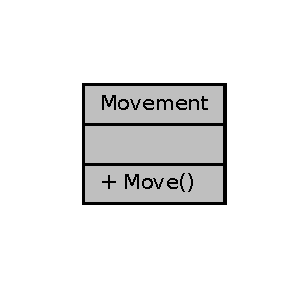
\includegraphics[width=148pt]{classMovement__coll__graph}
\end{center}
\end{figure}
\subsection*{Public Member Functions}
\begin{DoxyCompactItemize}
\item 
\mbox{\Hypertarget{classMovement_abfc624b2a9b15f9700c8684b5a079ba9}\label{classMovement_abfc624b2a9b15f9700c8684b5a079ba9}} 
virtual void \hyperlink{classMovement_abfc624b2a9b15f9700c8684b5a079ba9}{Move} (\hyperlink{classDrone}{Drone} \&drone, double direction\mbox{[}3\mbox{]}, double distance, float speed, double dt)=0
\begin{DoxyCompactList}\small\item\em Pure virtual function for handling drone movement. \end{DoxyCompactList}\end{DoxyCompactItemize}


\subsection{Detailed Description}
The class for handling movement of the drone. 

The documentation for this class was generated from the following file\+:\begin{DoxyCompactItemize}
\item 
/home/user/repo/project/src/movement.\+h\end{DoxyCompactItemize}

\hypertarget{classSimulation}{}\section{Simulation Class Reference}
\label{classSimulation}\index{Simulation@{Simulation}}


The class for simulating a drone finding a robot.  




{\ttfamily \#include $<$simulation.\+h$>$}



Inheritance diagram for Simulation\+:\nopagebreak
\begin{figure}[H]
\begin{center}
\leavevmode
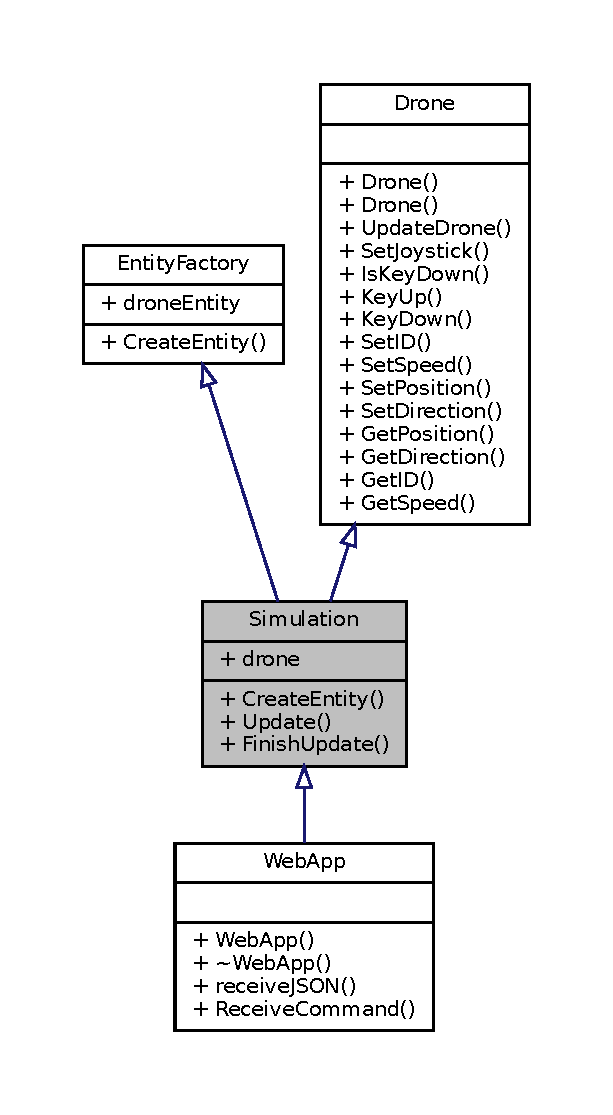
\includegraphics[width=294pt]{classSimulation__inherit__graph}
\end{center}
\end{figure}


Collaboration diagram for Simulation\+:\nopagebreak
\begin{figure}[H]
\begin{center}
\leavevmode
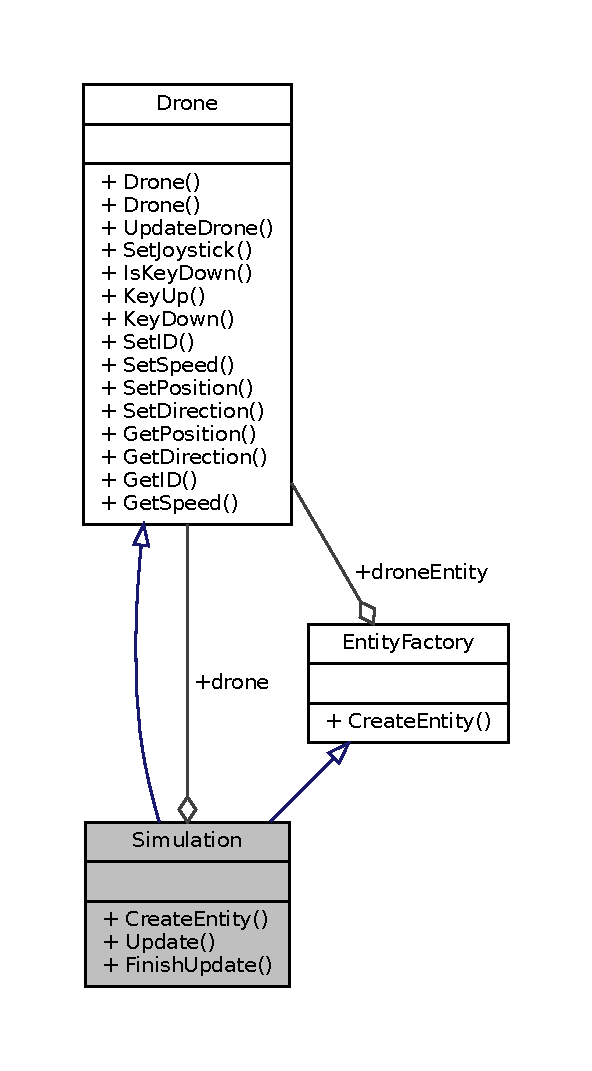
\includegraphics[width=284pt]{classSimulation__coll__graph}
\end{center}
\end{figure}
\subsection*{Public Member Functions}
\begin{DoxyCompactItemize}
\item 
\mbox{\Hypertarget{classSimulation_a3cd62ace1159d49c2120c2cf5d56e7ee}\label{classSimulation_a3cd62ace1159d49c2120c2cf5d56e7ee}} 
virtual void \hyperlink{classSimulation_a3cd62ace1159d49c2120c2cf5d56e7ee}{Create\+Entity} (picojson\+::object \&entity\+Data)
\begin{DoxyCompactList}\small\item\em Creates an entity based on object passed and sets all data fields. \end{DoxyCompactList}\item 
\mbox{\Hypertarget{classSimulation_a6f379a690fc567a53e74e954412467b0}\label{classSimulation_a6f379a690fc567a53e74e954412467b0}} 
void \hyperlink{classSimulation_a6f379a690fc567a53e74e954412467b0}{Update} (double dt)
\begin{DoxyCompactList}\small\item\em Updates the simulation based on time passed. \end{DoxyCompactList}\item 
\mbox{\Hypertarget{classSimulation_a073f3aa8c843e48b6b69148788d3fabf}\label{classSimulation_a073f3aa8c843e48b6b69148788d3fabf}} 
void \hyperlink{classSimulation_a073f3aa8c843e48b6b69148788d3fabf}{Finish\+Update} (picojson\+::object \&return\+Value)
\begin{DoxyCompactList}\small\item\em Updates the final display. Called after all updating is done. \end{DoxyCompactList}\end{DoxyCompactItemize}
\subsection*{Public Attributes}
\begin{DoxyCompactItemize}
\item 
\mbox{\Hypertarget{classSimulation_a215d77c2edb2dbcdad76658b020d00e5}\label{classSimulation_a215d77c2edb2dbcdad76658b020d00e5}} 
\hyperlink{classDrone}{Drone} {\bfseries drone} = Entity\+Factory\+::drone\+Entity
\end{DoxyCompactItemize}


\subsection{Detailed Description}
The class for simulating a drone finding a robot. 

The documentation for this class was generated from the following files\+:\begin{DoxyCompactItemize}
\item 
/home/user/repo/project/src/simulation.\+h\item 
/home/user/repo/project/src/simulation.\+cc\end{DoxyCompactItemize}

\hypertarget{classWebApp}{}\section{Web\+App Class Reference}
\label{classWebApp}\index{Web\+App@{Web\+App}}


A Web Application Sever that communicates with a web page through web sockets.  




{\ttfamily \#include $<$web\+\_\+app.\+h$>$}



Inheritance diagram for Web\+App\+:\nopagebreak
\begin{figure}[H]
\begin{center}
\leavevmode
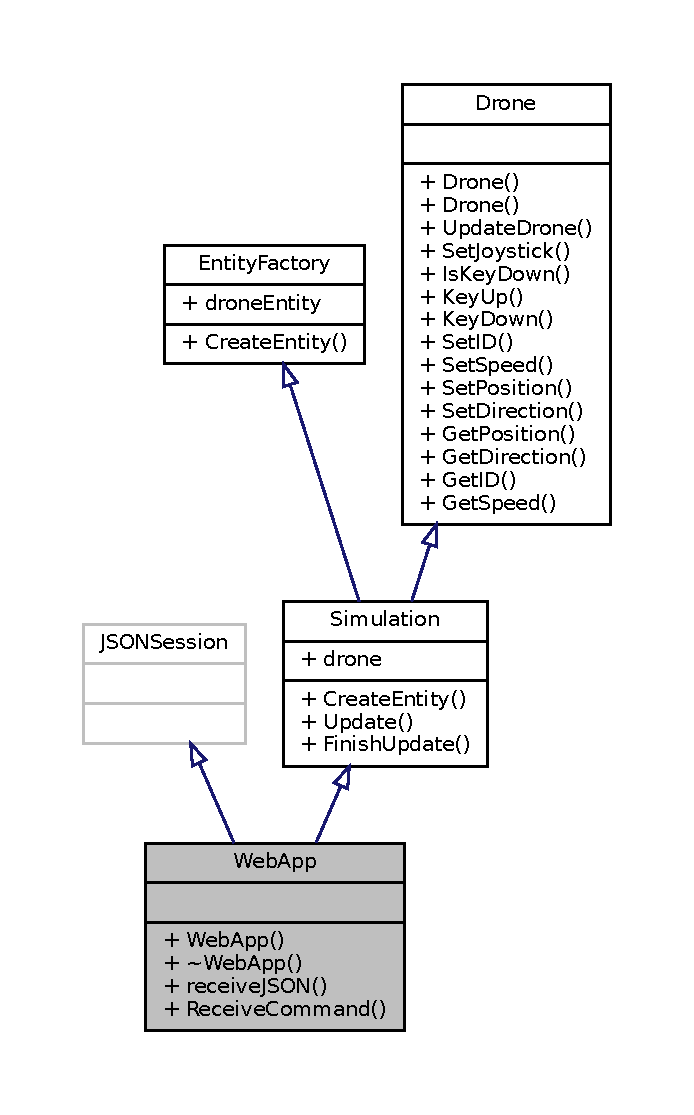
\includegraphics[width=333pt]{classWebApp__inherit__graph}
\end{center}
\end{figure}


Collaboration diagram for Web\+App\+:\nopagebreak
\begin{figure}[H]
\begin{center}
\leavevmode
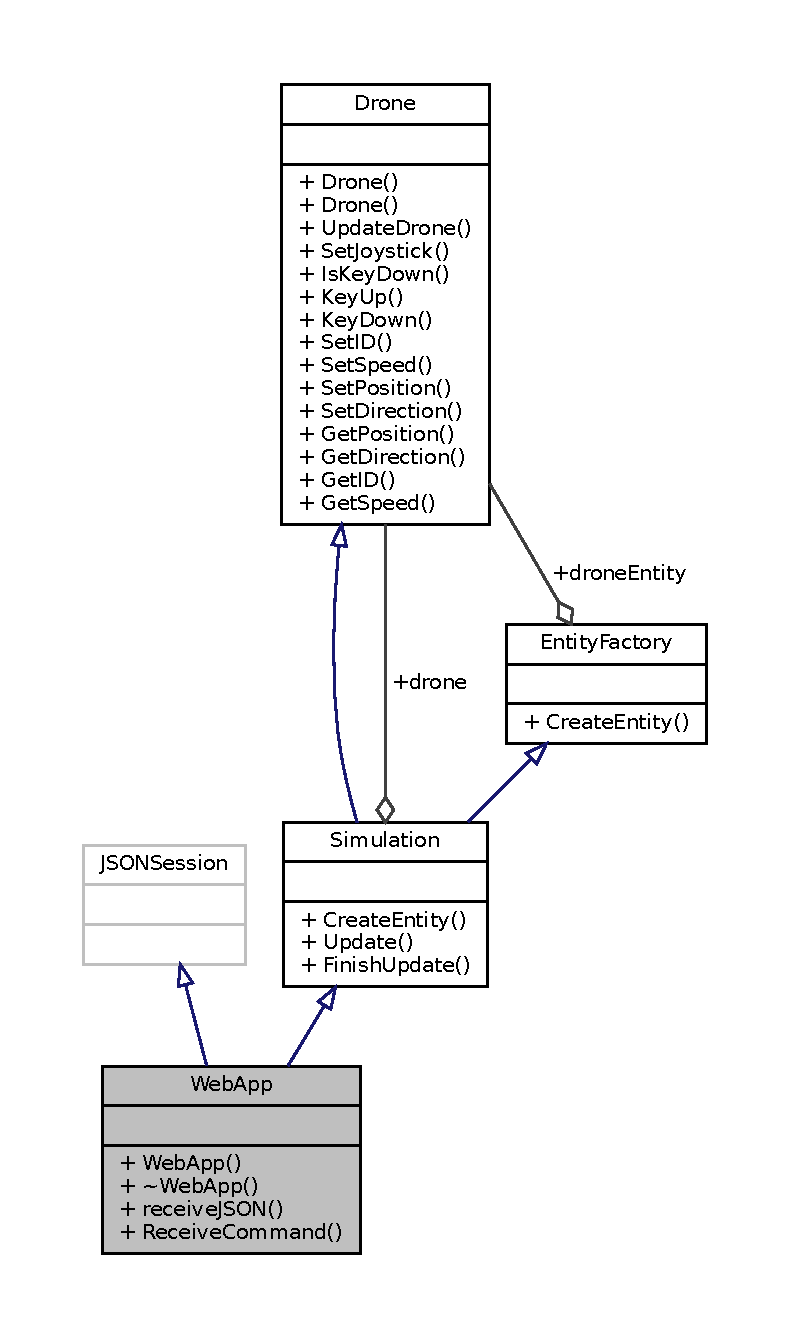
\includegraphics[height=550pt]{classWebApp__coll__graph}
\end{center}
\end{figure}
\subsection*{Public Member Functions}
\begin{DoxyCompactItemize}
\item 
\mbox{\Hypertarget{classWebApp_a9ba424099f42bdd456f52c4bba87d5b2}\label{classWebApp_a9ba424099f42bdd456f52c4bba87d5b2}} 
\hyperlink{classWebApp_a9ba424099f42bdd456f52c4bba87d5b2}{Web\+App} ()
\begin{DoxyCompactList}\small\item\em Initializes server. \end{DoxyCompactList}\item 
\mbox{\Hypertarget{classWebApp_ad73fb17d2f4176bb002a8e6df6346ef9}\label{classWebApp_ad73fb17d2f4176bb002a8e6df6346ef9}} 
virtual \hyperlink{classWebApp_ad73fb17d2f4176bb002a8e6df6346ef9}{$\sim$\+Web\+App} ()
\begin{DoxyCompactList}\small\item\em Destructor. \end{DoxyCompactList}\item 
\mbox{\Hypertarget{classWebApp_a0af5cfc12444f53e48609360eff95d76}\label{classWebApp_a0af5cfc12444f53e48609360eff95d76}} 
void \hyperlink{classWebApp_a0af5cfc12444f53e48609360eff95d76}{receive\+J\+S\+ON} (picojson\+::value \&val)
\begin{DoxyCompactList}\small\item\em Receives J\+S\+ON from the web server. \end{DoxyCompactList}\item 
\mbox{\Hypertarget{classWebApp_ac1ae360aa44aeb9f2bccb53f6d7881b4}\label{classWebApp_ac1ae360aa44aeb9f2bccb53f6d7881b4}} 
void \hyperlink{classWebApp_ac1ae360aa44aeb9f2bccb53f6d7881b4}{Receive\+Command} (const std\+::string \&cmd, picojson\+::object \&data, picojson\+::object \&return\+Value)
\begin{DoxyCompactList}\small\item\em Handles specific commands from the web server. \end{DoxyCompactList}\end{DoxyCompactItemize}
\subsection*{Additional Inherited Members}


\subsection{Detailed Description}
A Web Application Sever that communicates with a web page through web sockets. 

The documentation for this class was generated from the following files\+:\begin{DoxyCompactItemize}
\item 
/home/user/repo/project/src/web\+\_\+app.\+h\item 
/home/user/repo/project/src/web\+\_\+app.\+cc\end{DoxyCompactItemize}

%--- End generated contents ---

% Index
\backmatter
\newpage
\phantomsection
\clearemptydoublepage
\addcontentsline{toc}{chapter}{Index}
\printindex

\end{document}
